\chapter{Исследование системы управления тандемом с помощью имитационной модели}						% Заголовок
% \addcontentsline{toc}{chapter}{Исследование системы управления тандемом с помощью имитационной модели}	% Добавляем его в оглавление
% \setcounter{chapter}{4}
% \setcounter{section}{0}

Глава~4 имеет своей целью как подтвердить результаты, полученные аналитически в предыдущих главах, так и расширить их. С этой целью была разработана имитационная модель и написана программа для ее исследования. Для определения момента достижения системой стационарного режима подсчитываются различные статистики одновременно для двух систем: смещенной, то есть системы с ненулевым количеством требований в начале, и несмещенной, то есть системы с пустыми очередями при старте. Основным показателем качества работы системы выбрана средневзвешенная оценка времени пребывания требования в системе. В завершении главы приведены конкретные эксперименты и анализ их результатов.

\section{Описание имитационной модели}
Комплексные системы, состоящие из нескольких схожих или различных подсистем, могут рассматриваться с точки зрения понятия <<сложная система>>. Общее определение <<сложной системы>> было введено в работе \cite{Buslenko:1978} на основе изучения большого количества реальных комплексных систем и их математических моделей. Для анализа подобных систем ранее использовался весьма широкий математический аппарат: конечные автоматы, дифференциальные уравнения, динамические системы и теория массового обслуживания. Поэтому введение единого общего понятия представлялось актуальным и было осуществлено именно в работе \cite{Buslenko:1978}. Тандем управляющих систем обслуживания является одним из примеров таких <<сложных систем>>. 

До этой главы в работе исследовались свойства основных подсистем тандема: подсистемы с очередью низкоприоритетного потока, с очередями первичных входных потоков и с промежуточной очередью. Тем не менее, для всестороннего изучения системы необходимо также провести ее синтез. Другими словами, здесь и далее нас будет интересовать поведение системы в целом: ее эффективность и устойчивость с течением времени. Эффективность подобных систем может оцениваться, к примеру, с помощью одной из следующих характеристик: 1) среднее взвешенное количество ожидающих требований в очередях; 2) среднее взвешенное время нахождения в системе произвольного требования; 3) среднее взвешенное время ожидания в системе произвольного требования; 4) среднее время простоя системы. В данной работе акцент будет сделан на среднем взвешенном времени ожидания и средем взвешенном времени пребывания произвольного требования в системе.

% На базе математической модели тандема управляющих систем обслуживания построена имитационная модель для двух перекрестков (рис.~\ref{../Pictures/Crossroads.png}).

Математическая модель рассматриваемой в работе управляющей системы, построенная по принципам кибернетического подхода, существенно упростила построение и реализацию имитационной модели тандема перекрестков (рис.~\ref{crossroads}). В частности, нелокальное описание блоков системы помогло избежать формирования большого количества данных и, как следствие, их последующей обработки. Время имитации при этом должно существенно сократиться. Для смещенной и несмещенной систем в роли состояния выступали длины очередей и состояние обслуживающего устройства. В соответствии с законами распределения входных потоков  $\Pi_1$ и $\Pi_3$ генерировались требования системы. Для каждого требования фиксировался момент его прихода в систему, выхода из нее и время до обслуживания.

Альтернативным подходом к изложенному в этой работе является метод дискретных событий, подробно описанный в работах  \cite{AsmussenGlynn,Simulation} и использовавшийся, например, в работах \cite{FedotkinRachinskaya:2016,FedotkinADissertation}. В противовес нелокальному описанию системы, в роли наблюдаемых событий, как правило, выбирались вход в систему или выход из нее конкретного требования, момент смены обслуживающим устройством его состояния и т.д. В результате формируется исчерпывающее множество событий системы и создается полное описание всего процесса обслуживания. Поскольку для получения оценки основных характеристик работы системы такой объем информации является избыточным, то представляется целесообразным и зачастую необходимым отказаться от большей ее части.

В настоящей работе наибольший акцент при оценке эффективности работы системы делается на среднее взвешенное время нахождения произвольного требования первичных потоков $\Pi_1$ и $\Pi_3$ в системе: чем больше средняя интенсивность потока требований, тем больше вес требований этого потока. Время ожидания требований первичных потоков не характеризует процессов, происходящих между двумя перекрестками, поэтому в качестве конечного критерия эффективности работы не используется. Размер каждой очереди $O_j$, $j=\overline{1,4}$, сложно преобразовать в единую характеристику, поскольку очереди имеют качественно разную природу. Однако для определения момента наступления стационарного режима данная информация оказывается весьма полезной.

Опишем основные этапы работы программы. Изначально фиксируются параметры, определящие входные потоки:
$\lambda_j$,  $p_{\nu}^{(j)}>0$ ($j=1,3$, $\nu=1$, $2$, $\ldots$); параметры перекрестков: $\mu_1$, $\mu_2$,  $\mu_3$, $\mu_4$, $\mu_{\mathrm{prolong}}$; параметры алгоритма управления перекрестками: $\widetilde T^{(1,1)}$, $\widetilde T^{(1,2)}$, $\widetilde T^{(2,1)}$, $\widetilde T^{(2,2)}$, $\widetilde T^{(2,3)}$, $L$. Здесь величины $\mu_1$, $\mu_2$ и $\mu_3$  описывают интенсивности обслуживания требований потоков $\Pi_1$, $\Pi_2$ и $\Pi_3$ соответственно: $\ell(k,r,j)=[\mu_j T^{(k,r)}]$, если  поток $\Pi_j$ обслуживается и $\ell(k,r,j)=0$ если не обслуживается. А величина $\mu_{prolong}$ определяет интенсивность обслуживания требований потока $\Pi_2$ при продлении. Величина $\mu_4$ определяет вероятность $p_{k,r}$ для состояния $\Gamma^{(k,r)}$ продолжительностью $T^{(k,r)}$ по формуле $p_{k,r} = 1- \exp{(- T^{(k,r)} \mu_4)}$.  

%$\ell(k,r,j)=[\mu_j T^{(k,r)}]$, если  поток $\Pi_j$ обслуживается и $\ell(k,r,j)=0$ если не обслуживается. Величина $\mu_{\mathrm{prolong}}$ описывает интенсивность обуслуживания требований потока $\Pi_2$ при продлении. Величина $\mu_4$ определяет вероятность $p_{k,r}$ проезда автомобиля между перекрестками  для состояния $\Gamma^{(k,r)}$ продолжительностью $T^{(k,r)}$ по формуле $p_{k,r} = 1- \exp{(- T^{(k,r)} \mu_4)}$.  

Следующим шагом работы программы является объединение множеств состояний двух перекрестков и создание общего множества состояний для одной управляющей системы. При построении математической модели этот шаг описан достаточно детально. На выходе этого этапа также получаем граф переходов для обслуживающего устройства.

Имитация управляющей системы производится при двух различных начальных условиях. Первым начальным условием является полное отсутствие автомобилей в очередях к началу наблюдения за светофорами. В качестве второго условия выбирается случайное количество автомобилей для каждой очереди. В случае отсутствия требований в начальный момент времени, систему будем называть, следуя работе \cite{FedotkinRachinskaya:2016}, несмещенной и указывать индекс <<0>> при рассмотрении соотвествующих ей величин. В случае непустых очередей систему будем называть смещенной и соответствующие ей величины обозначать индексом <<+>>. Далее, для того, чтобы определить факт достижения системой стационарного режима используется информация о <<близости>> состояний смещенной и несмещенной систем. Непосредственный подсчет статистик, характеризующих качество работы управляющей системы, производится в стационарном режиме, после завершения переходных процессов. При записи величин, подсчитанных для стационарного режима, будем опускать индексы <<0>> и <<+>>.

Для изучения воздействия управляющих параметров на эффективность работы системы, изложенная выше процедура имитации выполняется для заранее заданной сетки значений. Сетка значений параметров выбиралась достаточно подробной для большей репрезентативности результатов. С другой стороны, множество значений не было избыточным для сокращения времени работы программы. 

\begin{figure}[t]
\centering
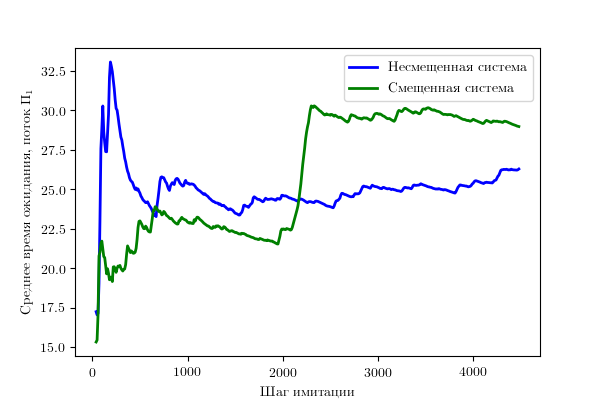
\includegraphics[scale=1]{Pictures/pic_firstTimeUntilServ_stationar.png} 
\caption{Динамика среднего времени ожидания произвольного требования потока $\Pi_1$. Система со стационарным режимом}
\label{Experiment:timeUntilServiceFirst:stationar}
\end{figure}

Основной текст программы написан на языке <<C++>> с использованием многофункционального расширяемого текстового редактора <<GNU Emacs $26.1$>> и компилятора <<GNU C++>> (<<g++>>) версии $7.3$. Для визуализации результатов имитационного моделирования использовался язык <<Python>> версии $3.6$. Подводя итог описанному выше алгоритму, программа включает в себя следующие компоненты.
\begin{itemize}
    \item Функция \textit{оптимизации}: 1) в соответствии с конфигурационным файлом формирует сетку управляющих параметров, с которыми будет запускаться имитационное моделирование; 2) для фиксированного набора параметров инициирует запуск имитации.
    \item Функция \textit{проверки стационарности} системы: 1) производит заданное количество итераций работы алгоритма для смещенной и несмещенной систем; 2) на каждой итерации проверяет близость характеристик смещенной и несмещенной систем и 3) фиксирует факт вступления систем в стационарный режим.
    \item Функция \textit{проведения итерации} системы: 1) осуществляет переключение состояний устройства и подсчет статистики их посещений; 2) осуществляет переключение состояний очередей и сбор статистик, связанных с размерами очередей; 3) с помощью генератора псевдослучайных чисел формирует значения величин, определяющих новые требования потоков $\Pi_1$ и $\Pi_3$, а также принимает решение об уже обслуженных требованиях.
    \item Функция \textit{оценки эффективности работы} системы: 1) аггрегирует характеристики эффективности, подсчитанные для несмещенной системы во время нахождения в стационарном режиме; 2) запись полученных результатов в файл и вывод необходимой информации на экран.
    \item Функция \textit{отрисовки результатов}: при помощи дополнительных модулей <<mpl\_toolkits>>, <<matplotlib>> языка <<Python>> формирует png-изображение, содержащее график результатов работы программы для различных управляющих параметров.
\end{itemize}

\begin{figure}[t]
\centering
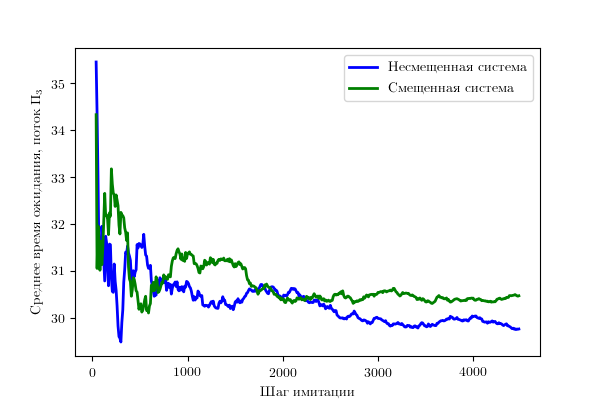
\includegraphics[scale=1]{Pictures/pic_secondTimeUntilServ_stationar.png} 
\caption{Динамика среднего времени ожидания произвольного требования потока $\Pi_3$. Система со стационарным режимом}
\label{Experiment:timeUntilServiceSecond:stationar}
\end{figure}
Опишем используемые в модели величины.
Зафиксируем индекс $j\in \{1, 3\}$, соответствующий номеру потока, и индекс $n=1$, $2$, $\ldots$, соответствующий очередному такту работы управляющей системы.

\begin{figure}[t]
\centering
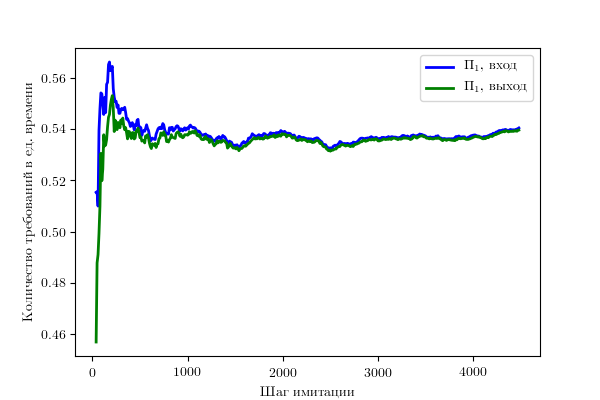
\includegraphics[scale=1]{Dissertation/Work_structured/Pictures/pic_inputOutputFirstFlow_stationar.png}
\caption{Динамика среднего числа поступивших и ушедших требований потока $\Pi_1$  за единицу времени. Система со стационарным режимом}
\label{Experiment:inputOutputFirstFlow:stationar}
\end{figure}
 При моделировании наблюдаются значения следующих статистик: $t_n$~--- продолжительность такта с номером $n$; $\gamma_{j,\nu}^+$ и $\gamma_{j,\nu}^0$~--- для смещенной и несмещенной систем соответственно время ожидания  автомобиля $\nu$ потока $\Pi_j$, $\nu=0$, $1$, $\ldots$;
 $\alpha^{+}_{\text{in},j,n}$ и $\alpha^{0}_{\text{in}, j,n}$~--- количество автомобилей потока $\Pi_j$, которые поступили за такт с номером $n$, в смещенной и несмещенной системах соответственно; 
 $\alpha^{+}_{\text{out},j,n}$ и $\alpha^{0}_{\text{out},j,n}$~--- количество автомобилей потока $\Pi_j$, которые закончили обслуживание на такте $n$ для смещенной и несмещенной систем соответственно;  $\zeta_{j,\nu}$~--- время, которое автомобиль с номером $\nu$ потока $\Pi_j$ провело с момента его прихода в систему и до момента его выхода; $\beta_{j,n}$~--- количество автомобилей, которые находятся в очереди $O_j$ при условии, что  очередь $O_j$ только что начала обслуживаться ($\beta_{j,n}=0$ в остальных случаях). Отметим, что время $\zeta_{1,\nu}$ нахождения в системе автомобиля потока $\Pi_1$ в том числе включает в себя время нахождения в системе его в качестве автомобиля потока $\Pi_2$ и потока $\Pi_4$. При совершении очередного события в системе происходит его обработка и изменение соответствующих отслеживаемых величин. В случае, если в течение определенного количества тактов (авторами экспериментально подобрано значение $100000$) стационарный режим в системе не обнаружен, то процесс имитации заканчивается. Однако, если система входит в стационарный режим, то в течение фиксированного количества тактов (авторами также экспериментально подобрано значение $100000$) происходит подсчет характеристик эффективности функционирования системы.




\begin{figure}[t]
\centering
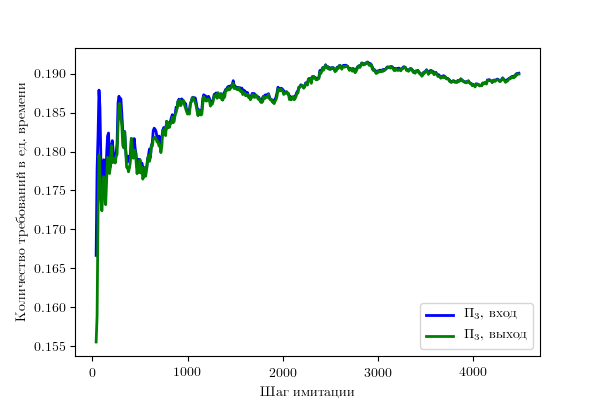
\includegraphics[scale=1]{Dissertation/Work_structured/Pictures/pic_inputOutputSecondFlow_stationar.png}
\caption{Динамика среднего числа поступивших и ушедших требований потока $\Pi_3$ за единицу времени. Система со стационарным режимом}
\label{Experiment:inputOutputSecondFlow:stationar}
\end{figure}

\section{Алгоритм определения момента достижения стационарного режима}
Как правило, под стационарным режимом на содержательном уровне понимают такой режим функционирования системы, устанавливающийся с течением времени, при котором выделенные ее характеристики в среднем остаются неизменными. Идея алгоритма определения момента достижения  такого режима в данной работе заключается в следующем. Наблюдаем одновременно за динамикой смещенной и несмещенной систем и считаем для каждой из них некоторые усредненные величины. Момент, когда эти величины станут достаточно близки, считаем моментом окончания переходных процессов. 

Детали алгоритма будем сопровождать результатами экспериментов, проведенных со следующими наборами параметров:
\begin{itemize}
    \item $\boldsymbol{\lambda_1\in \{0.3, 0.4\}}$, $p_{1}^{(1)}=0.4$, $p_{2}^{(1)}=0.4$, $p_{3}^{(1)}=0.2$, $p_{\nu}^{(1)}=0$, $\nu > 3$;
    \item $(\widetilde{T}^{(1,1)}, \widetilde{T}^{(1,2)})=(30,30)$, $\mu_1 = 1.2$, $\mu_2 = 1.3$;
    \item $\lambda_3=0.1$, $p_{1}^{(3)}=0.4$, $p_{2}^{(3)}=0.3$, $p_{3}^{(1)}=0.3$, $p_{\nu}^{(3)}=0$, $\nu > 3$;
        \item $\mu_4= 0.08$.
\end{itemize}
Здесь представлены два набора параметров, которые отличаются лишь значением параметра $\lambda_1$, выделенным жирным шрифтом. Причем случай $\lambda_1=0.3$ соответствует системе, для которой программно был зафиксирован стационарный режим, а случай $\lambda_1=0.4$~--- системе, для которой стационарный режим обнаружен не был.

\begin{figure}[t]
\centering
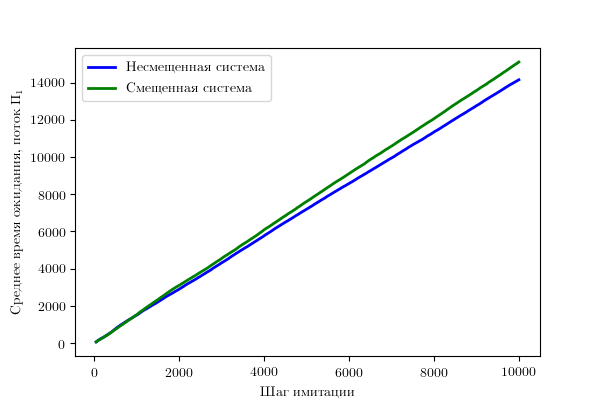
\includegraphics[scale=1]{Dissertation/Work_structured/Pictures/pic_firstTimeUntilServ.png}
\caption{Динамика среднего времени ожидания произвольного требования потока $\Pi_1$. Система без стационарного режима}
\label{Experiment:timeUntilServiceSecond:nonstationar}
\end{figure}

Перейдем к формализации алгоритма. Зафиксируем параметры метода:  $1 > \delta_1$, $1 < \delta_2$ и $1 < \delta_3$. В конце каждого такта будем считать значения 
\begin{equation}
   \gamma_{j,\cdot}^0 = \frac{1}{\tilde{\mathcal{V}}_j^0}\sum_{\nu} \gamma_{j,\nu}^0, \quad \gamma_{j,\cdot}^+ = \frac{1}{\tilde{\mathcal{V}}_j^+}\sum_{\nu} \gamma_{j,\nu}^+,
\end{equation}
среднего времени ожидания обслуживания требований потока $\Pi_j$, $j=1,3$, в несмещенной и смещенной системах соответственно. Динамика времен ожидания для конкретной системы со стационарным режимом при $\lambda_1=0.3$ приведена на рисунках \ref{Experiment:timeUntilServiceFirst:stationar} (для требований потока $\Pi_1$) и \ref{Experiment:timeUntilServiceSecond:stationar} (для требований потока $\Pi_3$).



Для большей устойчивости алгоритма принятия решения о наступлении стационарного режима в несмещенной системе будем следить за количеством требований во входящем и выходящем потоков:
\begin{equation}
    F^{0}_{\text{in},1} = \sum_n \alpha^{0}_{\text{in},1,n}, \quad 
    F^{0}_{\text{out},4} = \sum_n \alpha^{0}_{\text{out},4,n},
\end{equation}
\begin{equation}
    F^{0}_{\text{in},3} = \sum_n \alpha^{0}_{\text{in},3,n}, \quad 
    F^{0}_{\text{out},3} = \sum_n \alpha^{0}_{\text{out},3,n}.
\end{equation}
Для системы со стационарным режимом ожидается, что среднее число требований, пришедших в систему в единицу времени, $F^{0}_{\text{in},1}$ и $F^{0}_{\text{in},3}$, не будет существенно превышать среднее число требований, $ F^{0}_{\text{out},4}$ и $F^{0}_{\text{out},3}$ соответственно, покинувших систему за единицу времени. Поскольку при поступлении в систему требования потока $\Pi_1$ проходят дополнительные этапы обслуживания~--- в качестве требований потока $\Pi_2$ и $\Pi_4$,~--- то количество требований потока $\Pi_1$, покинувших систему, целесообразно считать по выходному потоку $\Pi_4^{\text{out}}$. Динамика соответствующих величин представлена на рисунках \ref{Experiment:inputOutputFirstFlow:stationar} и \ref{Experiment:inputOutputSecondFlow:stationar}.

\begin{figure}[t]
\centering
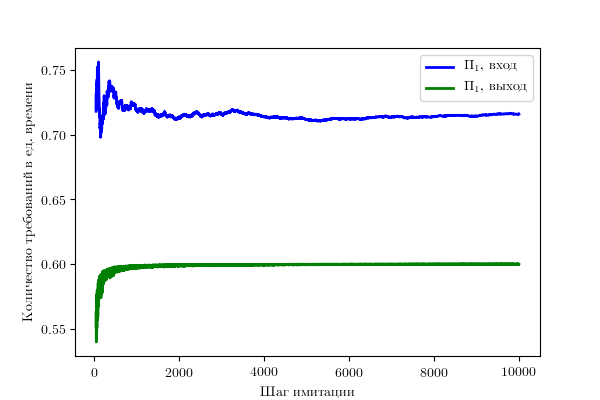
\includegraphics[scale=1]{Dissertation/Work_structured/Pictures/pic_inputOutputFirstFlow.png}
\caption{Динамика среднего числа поступивших и ушедших требований потока $\Pi_3$ за единицу времени. Система со стационарным режимом}
\label{Experiment:inputOutputFirstFlow}
\end{figure}




Окончательное решение о достижении системой стационарного режима будет приниматься в случае, если выполнены следующие неравенства:
\begin{equation}
    \frac{|\gamma_{j,\cdot}^0 - \gamma_{j,\cdot}^+|}{\gamma_{j,\cdot}^0} < \delta_1, \quad
    \frac{F^{0}_{\text{in},1}}{F^{0}_{\text{out},4}} < \delta_2, \quad 
    \frac{F^{0}_{\text{in},3}}{F^{0}_{\text{out},3}} < \delta_3.
\end{equation}

Рассмотрим систему, в которой некоторые очереди неограниченно возрастают и, следовательно, стационарный режим достигнут быть не может. Проанализируем динамику среднего времени ожидания произвольного требования в смещенной и несмещенной системах (рис.~\ref{Experiment:timeUntilServiceSecond:nonstationar}).  Как видно из рисунка, величины $\gamma_{j,\cdot}^0$ и $ \gamma_{j,\cdot}^+$ неограниченно возрастают, причем с похожей скоростью. Поэтому величина $\frac{|\gamma_{j,\cdot}^0 - \gamma_{j,\cdot}^+|}{\gamma_{j,\cdot}^0} $ будет небольшой за счет большого знаменателя и относительно небольшого числителя. 


\begin{figure}[h]
\centering
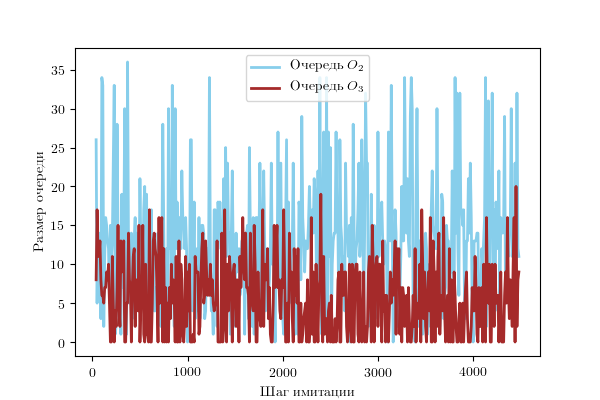
\includegraphics[scale=1]{Dissertation/Work_structured/Pictures/pic_queues_2_stationar.png}
\caption{Динамика длин очередей $O_2$ и $O_3$ второго перекрестка. Система со стационарным режимом}
\label{Experiment:queues:2:stationar}
\end{figure}
Для учета подобных случаев при фиксации факта наличия или отсутствия стационарного режима использовались средние количества входящих и выходящих требований в единицу времени по потокам $\Pi_1$ и $\Pi_3$. Динамика соответствующих величин $F^{0}_{\text{in},1}$ и $F^{0}_{\text{out},4} $ для потока $\Pi_1$ представлена на рисунке~\ref{Experiment:inputOutputFirstFlow}. Из графика видно, что количество $F^{0}_{\text{in},1}$ входящих требований в единицу времени заметно превышает количество $F^{0}_{\text{out},4}$ выходящих требований в единицу времени, поэтому неравенство $\frac{F^{0}_{\text{in},1}}{F^{0}_{\text{out},4}} < \delta_2$ не сможет быть выполнено. 


\section{Показатели качества работы системы}
Как было сказано ранее, важнейшими характеристиками работы системы являются размер очередей и средние времена нахождения требований в системе. Здесь, как и в предыдущем пункте, в качестве примера будем рассматривать запуски программ с теми же двумя наборами параметров, отличающиеся лишь параметром $\Lambda_1$. Для системы со стационарным режимом динамика длин очередей второго перекрестка $O_2$ и $O_3$ представлена на рисунке~\ref{Experiment:queues:2:stationar}. Динамика длины очереди первого перекрестка $O_1$ и длины промежуточной очереди $O_4$ представлены на рисунке~\ref{Experiment:queues:1:stationar}.

\begin{figure}[h]
\centering
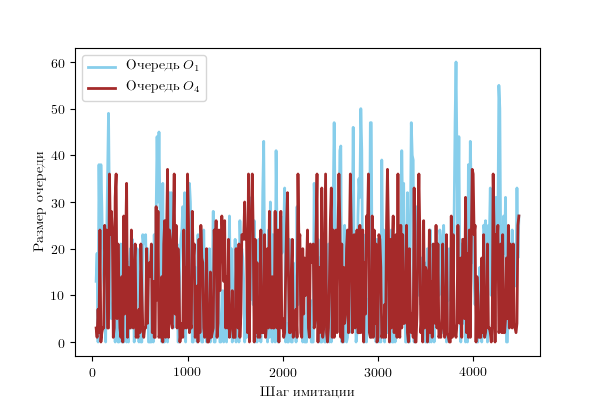
\includegraphics[scale=1]{Dissertation/Work_structured/Pictures/pic_queues_1_stationar.png}
\caption{Динамика длины очереди первого перекрестка $O_1$ и длины промежуточной очереди $O_4$. Система со стационарным режимом}
\label{Experiment:queues:1:stationar}
\end{figure}
Как видно из графиков, длины очередей колеблются между нулем и некоторым конечным числом, что <<подсказывает>> о существовании в такой системе стационарного режима.

%
С другой стороны, при наблюдении за длинами очередей в системе без стационарного режима, величина некоторых очередей может неограниченно возрастать (см. рис.~\ref{Experiment:queues:1:nonstationar}).
\begin{figure}[h]
\centering
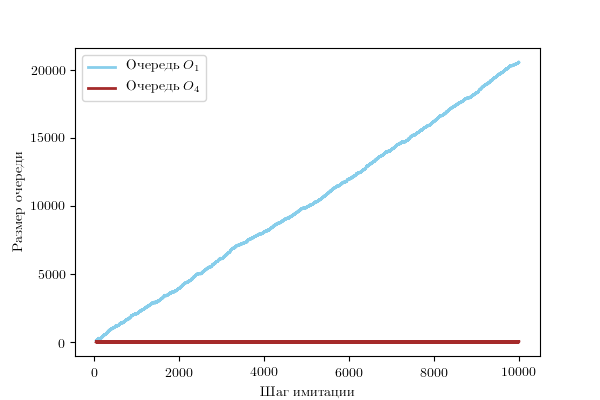
\includegraphics[scale=1]{Dissertation/Work_structured/Pictures/pic_queues_1.png}
\caption{Динамика длины очереди первого перекрестка $O_1$ и длины промежуточной очереди $O_4$. Система без стационарного режима}
\label{Experiment:queues:1:nonstationar}
\end{figure}

После того, как стационарный режим в системе достигнут, можно приступать к оценке основных показателей качества функционирования системы. С этой целью продолжается процесс имитации, но только для несмещенной системы. Необходимо получить оценки для математического ожидания времени пребывания произвольного требования потока $\Pi_j$, $j\in \{1, 3\}$.
%и математического ожидания количества требований в очереди $O_j$ в момент перехода обслуживающего устройства в состояние $^j\Gamma$ на произвольном цикле стационарного режима работы системы. 
За основу можно взять известные в теории вероятностей и математической статистике оценки соответствующих количественных характеристик. Оценки для времени пребывания в системе можно было бы построить по наблюдениям за каждым обслуженным требованием выделенной реализации потока $\Pi_j$.
%, а оценки для количества требований в очереди при переходе к состоянию обслуживания -- по наблюдениям за этой величиной на каждом цикле одной реализации. 
Итак, для каждого $j=1,3$  предлагаются следующие оценки для показателей качества работы системы по потоку $\Pi_j$ :
\begin{itemize}
    \item $\hat{E}\gamma_{j}=\frac{1}{\tilde{\mathcal{V}}_j}\sum_{\nu}\zeta_{j,\nu}$  -- оценка математического ожидания времени пребывания в системе произвольного требования потока $\Pi_j$.
\end{itemize}
Динамика среднего времени пребывания в системе для рассматриваемого примера изображена на рисунке~\ref{Experiment:serv:stationar}.
\begin{figure}[h]
\centering
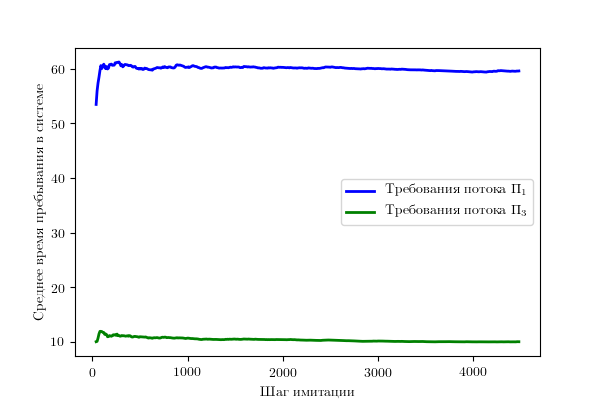
\includegraphics[scale=1]{Dissertation/Work_structured/Pictures/pic_serv_1_stationar.png}
\caption{Динамика среднего времени пребывания требований в системе. Система со стационарным режимом}
\label{Experiment:serv:stationar}
\end{figure}
%
Кроме того, имеет смысл получить оценки, характеризующие работу системы не по отдельному потоку, а для системы в целом. Для этого предлагается строить средние взвешенные оценки, где в качестве веса отдельному потоку приписывается интенсивность поступления его требований, т.е. величина, равная $\lambda_j \sum_{\nu\geqslant1}\nu p_{\nu}^{(j)}$. Итак, имеем результирующую оценку целевой функции
\begin{itemize}
    \item $\hat{E}\gamma=\frac{\sum_{j\in\{1,3\}} (\lambda_j \sum_{\nu\geqslant1}\nu p_{\nu}^{(j)})\hat{E}\gamma_{j} }{\sum_{j\in\{1,3\}} \lambda_j \sum_{\nu\geqslant1}\nu p_{\nu}^{(j)}}$.
\end{itemize}


\section{Анализ области стационарности системы}
Для анализа функционирования тандема перекрестков были зафиксированы следующие параметры:
\begin{itemize}
    \item $\lambda_1=0.35$, $p_{1}^{(1)}=0.4$, $p_{2}^{(1)}=0.4$, $p_{3}^{(1)}=0.2$, $p_{\nu}^{(1)}=0$, $\nu > 3$;
    \item $(\widetilde{T}^{(1,1)}, \widetilde{T}^{(1,2)})=(20,10)$, $\mu_1 = 1.2$;
    \item $\boldsymbol{ \lambda_3=\{0.1, 0.2\}}$, $p_{1}^{(3)}=0.4$, $p_{2}^{(3)}=0.3$, $p_{3}^{(1)}=0.3$, $p_{\nu}^{(3)}=0$, $\nu > 3$;
        \item $\mu_4= 0.001$.
\end{itemize}
Данные наборы параметров уже упоминались выше. Здесь представлены два набора параметров, отличающихся лишь интенсивностью $\boldsymbol{\lambda_3}$ поступления групп требований по потоку $\Pi_3$. Для алгоритма управления перекрестками зафиксируем длительность $\widetilde{T}^{(2,3)}=10$ продления зеленого сигнала светофора для потока $\Pi_2$ и порог $L=10$ продления.

При фиксированном наборе параметров ($\lambda_3 = 0.1$ либо $\lambda_3=0.2$) проводилась серия экспериментов, в которых перебирались значения для длительности обслуживания  $\widetilde{T}^{(2,1)} = \{1, 5, 9, \ldots, 97\}$ требований потока $\Pi_3$ и длительности обслуживания $\widetilde{T}^{(2,2)} = \{1, 5, 9, \ldots, 97\}$ потока $\Pi_2$.

%0_1_thres_10_target
\begin{figure}[h]
\centering
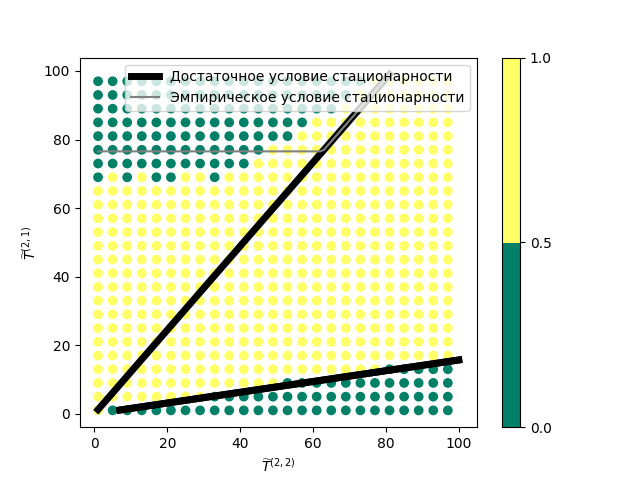
\includegraphics[scale=0.85]{Pictures/0_1_thres_10_target_fact.png} 
\caption{Области стационарности системы. $\lambda_3=0.1$, $L=10$}
\label{Experiment:stationar}
\end{figure}
На рис.~\ref{Experiment:stationar} представлены результаты экспериментов. По осям координат отложены значения $\widetilde T^{(2,1)}$ длительности обслуживания требований потока $\Pi_3$ и значения $\widetilde T^{(2,2)}$ длительности обслуживания требований потока $\Pi_2$. Желтым цветом обозначены точки, в которых было определено достижение системой стационарного режима. Темно-зеленым цветом обозначены случаи отсутствия стационарности. Кроме того на графике черным цветом изображены границы области стационарности, полученная из достаточных условий теоремы~\ref{sufficient:double:theorem}. 

Из графика видно, что желтая область выходит далеко за границы черных линий. Это свидетельствует о том, что достаточное условие, полученное в работе аналитически, не является необходимым. Ввод дополнительного режима продления по высоко приоритетному потоку при отсутвии большого числа требований по низкоприоритетному потоку позволяет существенно расширить область стационарности системы. Интуитивно данный результат ожидаем: при отсутствии требований по одному из потоков, другой поток получает дополнительный временной <<запас>> для обслуживания за счет продления.

Также на графике изображена область, ограниченная серой линией. Эта область получена эмпирическими рассуждениями и дает <<примерную>> оценку области стационарности для системы с продлением. Рассуждения для вывода этой границы основаны на подсчете <<среднего>> количества времени, освобождающегося для обслуживания требований потока $\Pi_2$ за счет продления.

\begin{figure}[h]
\centering
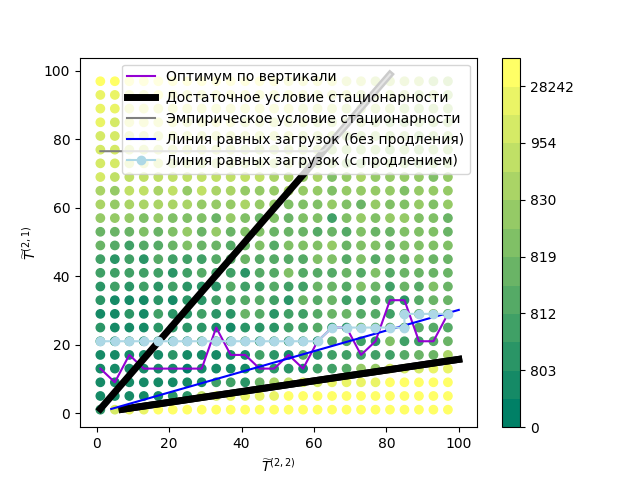
\includegraphics[scale=0.9]{Pictures/0_1_thres_10_target.png} 
\caption{Поиск оптимальных параметров системы}
\label{Experiment:targets}
\end{figure}


Более детально результаты эксперимента представлены на рис.~\ref{Experiment:targets}. На этом рисунке каждому эксперименту соответствует посчитанная оценка средневзвешенной длительности ожидания одного требования. Чем более темным является цвет точки~--- тем лучше. Кроме присутствовавших на предыдущем рисунке границ, здесь присутствуют линии равных загрузок для случая циклического управления (синий цвет) и для случая циклического управления с продлением (голубой цвет). В работах \cite{Fedotkin:2009} и \cite{FedotkinRachinskaya:2016} было отмечено, что оптимальные значение параметров с точки зрения средневзвешенного времени пребывания находится вблизи ломаной равных загрузок. При условии отсутствия продления ($\widetilde T^{(2,3)}=0$),  под загрузкой системы, например, по потоку $\Pi_1$ естественно понимать величину
\begin{equation}
\frac{(\widetilde T^{(2,1)} + \widetilde T^{(2,2)})\lambda_1 \sum_{\nu\geqslant 1}\nu p_{\nu}^{(1)}}{[\mu_2 \widetilde T^{(2,2)}]}.
\end{equation}
Тогда ломаную равных загрузок определим из условия равенства загрузки системы по потокам $\Pi_1$ и $\Pi_3$:
\begin{equation}
\frac{(\widetilde T^{(2,1)} +\widetilde T^{(2,2)})\lambda_1 \sum_{\nu\geqslant 1}\nu p_{\nu}^{(1)}}{[\mu_2 \widetilde T^{(2,2)}]}=
    \frac{(\widetilde T^{(2,1)} + \widetilde T^{(2,2)})\lambda_3 \sum_{\nu\geqslant 1}\nu p_{\nu}^{(3)}}{[\mu_3 \widetilde T^{(2,1)}]}
\end{equation}
График этой кривой изображен на рисунке~\ref{Experiment:targets} синим цветом. 

Далее встает вопрос о том, что считать загрузкой системы в случае присутствия продления по низкоприоритетному потоку $\Pi_3$. В данной работе под загрузкой будем понимать отношение общего числа пришедших требований по потоку ($\Pi_1$ или $\Pi_3$) к общему числу обслуженных требований по этому потоку. Аналитически посчитать эти величины сложно, поэтому на графике представлена кривая равных загрузок, посчитанная на основе экспериментальных данных. Как видно из рисунка, такая кривая лучше <<следует>> за оптимальными значениями параметров, нежели кривая равных загрузок для циклического алгоритма.
\begin{figure*}
\begin{multicols}{2}
    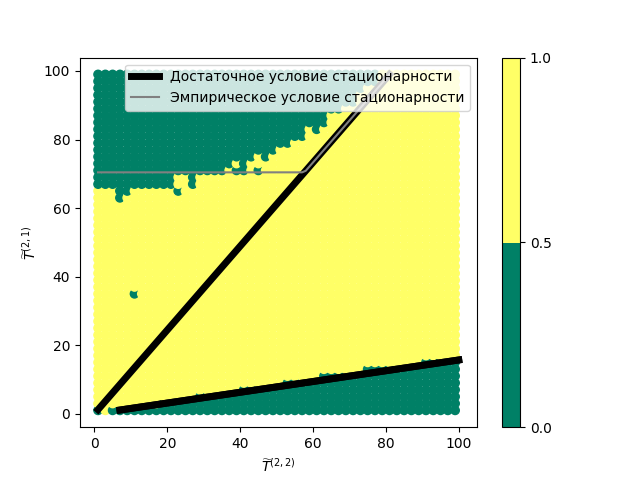
\includegraphics[width=1.2\linewidth]{Pictures/0_1_thres_10_fact.png}\par 
    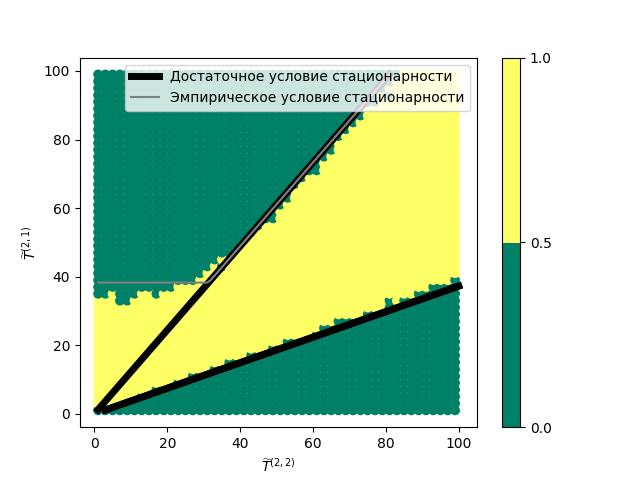
\includegraphics[width=1.2\linewidth]{Pictures/0_2_thres_10_fact.png}\par 
    \end{multicols}
\caption{Области стационарности для разных значений $\lambda_1$. Слева $\lambda_1=0.1$, справа $\lambda_1=0.2$}
\label{Experiment:intensities}
\end{figure*}

Поясним, что значит кривая равных загрузок лучше <<следует>> за оптимальными значениями параметров. Поставим задачу при фикисированном значении времени обслуживания потока $\Pi_2$ (величина $\widetilde T^{(2,2)}$ на рис.~\ref{Experiment:targets}) найти такое значение времени обслуживания потока $\Pi_3$ (величина $\widetilde T^{(2,1)}$ на рис.~\ref{Experiment:targets}), при котором достигается минимум средневзвешенного времени пребывания требования в системе. Фиолетовая линия на рис.~\ref{Experiment:targets} демонстрирует динамику этих значений при изменении времен $\widetilde T^{(2,2)}$. Видно, что <<в среднем>> голубая линия лучше аппроксимирует фиолетовую кривую, чем синяя. Особенно в окрестности прямой $\widetilde T^{(2,2)}=0$. 

\begin{figure*}
\begin{multicols}{2}
    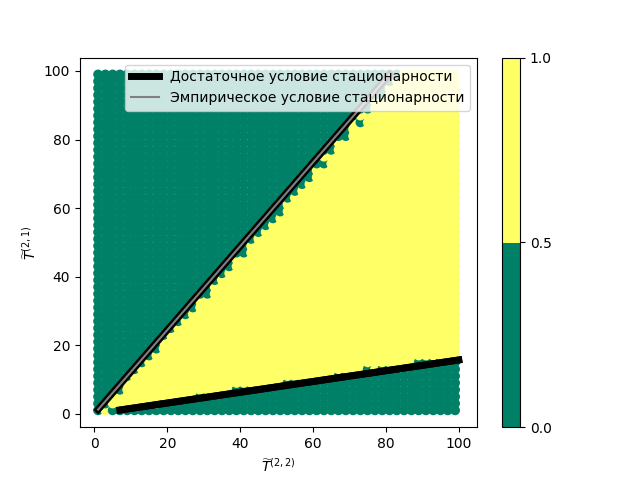
\includegraphics[width=1.15\linewidth]{Pictures/0_1_thres_-1_fact.png}\par 
    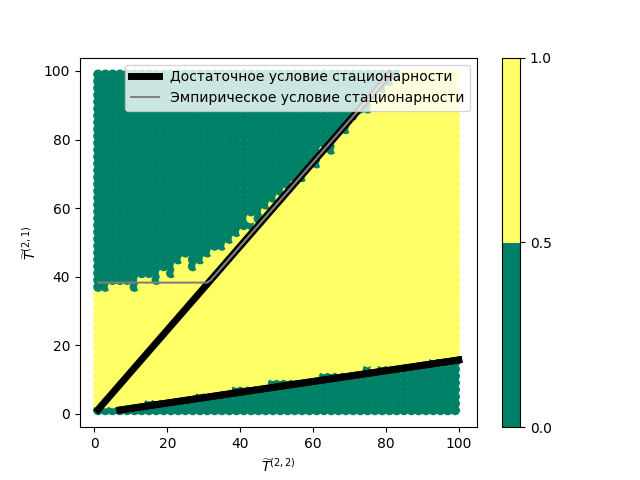
\includegraphics[width=1.15\linewidth]{Pictures/0_1_thres_5_fact.png}\par 
    \end{multicols}
\begin{multicols}{2}
    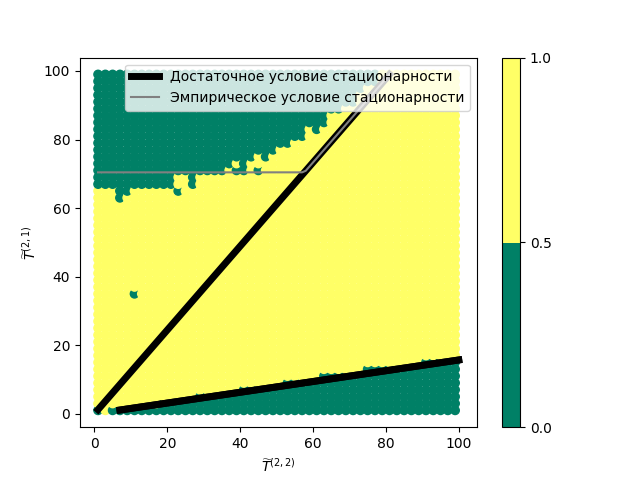
\includegraphics[width=1.15\linewidth]{Pictures/0_1_thres_10_fact.png}\par
    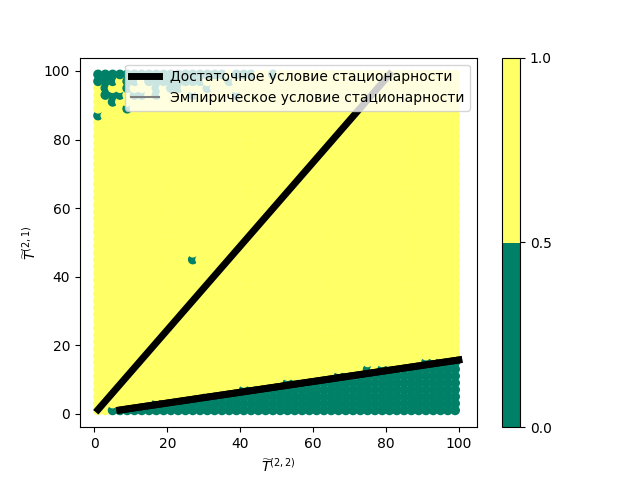
\includegraphics[width=1.15\linewidth]{Pictures/0_1_thres_15_fact.png}\par
\end{multicols}
\caption{Области стационарности для разных значений $L$. Слева-направо, сверху-вниз $L=-1$; $5$; $10$; $15$}
\label{different:thres}
\end{figure*}
Завершая анализ экспериментальных данных, отметим следующее.
\begin{itemize}
    \item При увеличении интенсивности потока $\Pi_2$ (или, что то же самое, интенсивности потока $\Pi_1$), область стационарности сужается (см.~рис.~\ref{Experiment:intensities}).
    \item С увеличением порога $L$ продления, область стационарности увеличивается (см.~рис.~\ref{different:thres}).
\end{itemize}

